% !TEX encoding = UTF-8 Unicode
%%% Template originaly created by Karol Kozioł (mail@karol-koziol.net) and modified for ShareLaTeX use
\documentclass[a4paper,11pt]{article}
\usepackage[french]{babel} % English language/hyphenation
\usepackage{mathptmx} % Use the Adobe Times Roman as the default text font together with math symbols from the Sym­bol, Chancery and Com­puter Modern fonts

\usepackage[T1]{fontenc}
\usepackage{ucs}
\usepackage[utf8x]{inputenc}
\usepackage{lipsum} % Inserts dummy text
\usepackage{graphicx}
\usepackage{color}

\renewcommand\familydefault{\sfdefault}
\usepackage{tgheros}
%\usepackage[defaultmono]{droidmono}

\usepackage{amsmath,amsfonts,amssymb,amsthm} % For math equations, theorems, symbols, etc
\usepackage{enumerate}
\usepackage{multicol}
\usepackage{tikz}
\usepackage[tikz]{bclogo}
\usepackage{multicol}
\usepackage{geometry}
\geometry{total={210mm,297mm},
left=25mm,right=25mm,%
bindingoffset=0mm, top=20mm,bottom=20mm}
\usepackage{url}
\usepackage[linkbordercolor=blue]{hyperref}
\author{M. A. Ammar - IPEST : HAP}
\date{16 décembre 2020}
\setlength{\parindent}{0pt}



\linespread{1.3}

\newcommand{\linia}{\rule{\linewidth}{0.5pt}}

% custom theorems if needed
\newtheoremstyle{mytheor}
    {1ex}{1ex}{\normalfont}{0pt}{\scshape}{.}{1ex}
    {{\thmname{#1 }}{\thmnumber{#2}}{\thmnote{ (#3)}}}

\theoremstyle{mytheor}
\newtheorem{defi}{Definition}

% my own titles
\makeatletter
\renewcommand{\maketitle}{
\begin{center}
\vspace{2ex}
{\huge \textsc{\@title}}
\vspace{1ex}
\\
\linia\\
\@author \hfill \@date
\vspace{4ex}
\end{center}
}
\makeatother
%%%

% custom footers and headers
\usepackage{fancyhdr}
\pagestyle{fancy}
\lhead{}
\chead{}
\rhead{}
\lfoot{}
\cfoot{}
\rfoot{Page \thepage}
\renewcommand{\headrulewidth}{0pt}
\renewcommand{\footrulewidth}{0pt}

%%%%%%%%%%%%%%%%%%%%%%%%%%%%%%%%%%%%%%%%
%%%%%%%%%%%%%%%%%%%%%%%%%%%%%%%%%%%%%%%%%
%%%% CODE
%%%%%%%%%%%%%%%%%%%%%%%%%%%%%%%%%%%%%%%%
\usepackage{fancyvrb} % packages needed for verbatim environments
\usepackage{listingsutf8}

\definecolor{mygreen}{rgb}{0,0.6,0}
\definecolor{mygray}{rgb}{0.5,0.5,0.5}
\definecolor{mymauve}{rgb}{0.58,0,0.82}
\DeclareFixedFont{\ttb}{T1}{pcr}{bx}{n}{10} % for bold
\DeclareFixedFont{\ttm}{T1}{pcr}{m}{n}{10}  % for normal
\lstset{ 
	backgroundcolor=\color{lightgray!10},   % choose the background color; you must add \usepackage{color} or \usepackage{xcolor}; should come as last argument
	basicstyle=\ttm,        % the size of the fonts that are used for the code
	breakatwhitespace=false,         % sets if automatic breaks should only happen at whitespace
	breaklines=true,                 % sets automatic line breaking
	postbreak=\raisebox{0ex}[0ex][0ex]{\ensuremath{\color{red}\hookrightarrow\space}},
	captionpos=b,                    % sets the caption-position to bottom
	commentstyle=\color{mygreen},    % comment style
	deletekeywords={...},            % if you want to delete keywords from the given language
	escapeinside={\%*}{*)},          % if you want to add LaTeX within your code
	extendedchars=true,              % lets you use non-ASCII characters; for 8-bits encodings only, does not work with UTF-8
	firstnumber=1,                % start line enumeration with line 1000
	frameround=fttt,
	frame=single,	                   % adds a frame around the code
	keepspaces=true,                 % keeps spaces in text, useful for keeping indentation of code (possibly needs columns=flexible)
	keywordstyle=\ttb\color{blue},       % keyword style
	language=Python,                 % the language of the code
	morekeywords={*,...},            % if you want to add more keywords to the set
	numbers=left,                    % where to put the line-numbers; possible values are (none, left, right)
	numbersep=5pt,                   % how far the line-numbers are from the code
	numberstyle=\tiny\color{mygray}, % the style that is used for the line-numbers
	rulecolor=\color{black},         % if not set, the frame-color may be changed on line-breaks within not-black text (e.g. comments (green here))
	showspaces=false,                % show spaces everywhere adding particular underscores; it overrides 'showstringspaces'
	showstringspaces=false,          % underline spaces within strings only
	showtabs=false,                  % show tabs within strings adding particular underscores
	stepnumber=1,                    % the step between two line-numbers. If it's 1, each line will be numbered
	stringstyle=\color{mymauve},     % string literal style
	tabsize=4,	                   % sets default tabsize to 2 spaces
	title=\lstname                   % show the filename of files included with \lstinputlisting; also try caption instead of title
}
\usepackage{textcomp}
\DefineVerbatimEnvironment % create new one
{pyshell}{Verbatim}{frame=leftline, framerule=1.5mm, rulecolor=\color{blue}}
\begin{document}
	
\title{Épreuve d'informatique (Python) \textnumero 1 \\ Durée : \texttt{1h 30'}}

\maketitle
\begin{bclogo}[logo=\bcattention, couleurBarre=red, noborder=true, couleur=red!10]{Documents non autorisés.}
\begin{itemize}
\item L'épreuve comporte 3 pages.
\item La présentation, la lisibilité, la qualité de la rédaction et la précision des raisonnements entreront pour une part importante dans l'appréciation des copies.
\item  Les algorithmes doivent être commentés.
\end{itemize}

\end{bclogo}
\section*{Exercice 1 : Calculer les niveaux d'énergie dans un atome}
Le $n^{ième}$ niveau d'énergie d'un électron dans un atome d'hydrogène est donné par:
\begin{equation}
E_n = -\frac{m_e e^4}{8\epsilon_0^2h^2}\cdot\frac{1}{n^2} ,
\end{equation}
où $m_e = 9.1094⋅10^{-31} \ kg$ est la masse de l'électron, $e = 1.602210^{−19} \ C$ est la charge élémentaire, $\epsilon_0 = 8.8542 \cdot 10^{-12} C^2 s^2 \ kg^{-1}m^{-3}$ est la permittivité électrique du vide, et $h=6.6261 \cdot 10^{−34} \ Js$


\begin{itemize}
\item[\textbf{Q1.}] Écrire la fonction \texttt{E(n)} qui retourne la valeur du niveau d'énergie en électron-volt ($eV$).


\begin{bclogo}[logo=\bclampe, couleurBarre=green, noborder=true, couleur=yellow!10]{Indications.}
On vous rappelle que $1 \ eV = 1.6022 \dot 10^{-19} \ J$.
\end{bclogo}

\item[\textbf{Q2.}] Calculer la valeur du niveau d'énergie le plus bas, \texttt{E(n=1)}. A quoi correspond ce niveau d'énergie?

\item[\textbf{Q3.}] Tester la valeur du niveau d'énergie pour $n \rightarrow \infty$. A quoi correspond le niveau d'énergie $E = 0$ eV ?

\item[\textbf{Q4.}] Écrire une boucle qui calcule et affiche le niveau d'énergie $E_n$ pour $n = 1,\dots, 20$.

\begin{bclogo}[logo=\bclampe, couleurBarre=green, noborder=true, couleur=yellow!10]{Indications.}
Le résultat doit être comme suivant:
\begin{pyshell}
E1 = -13.606152702370753 eV
E2 = -3.4015381755926883 eV
............................
............................
E19 = -0.03769017369077771 eV
E20 = -0.03401538175592689 eV
\end{pyshell}
\end{bclogo}
\item[\textbf{Q5.}] L'énergie libérée lorsqu'un électron se déplace du niveau ni au niveau nf est donnée par:
\begin{equation}
\Delta E = -\frac{m_e e^4}{8\epsilon_0^2h^2}\cdot\left( \frac{1}{n_i^2}-\frac{1}{n_f^2}\right)
\end{equation}
Construire et afficher la liste qui représente la matrice $\Delta E^{i,f}$ dont la cellule de la colonne \texttt{i} et de la ligne \texttt{f} contient l'énergie libérée lorsqu'un électron passe du niveau d'énergie \texttt{i} au niveau \texttt{f}, pour $i, f = 1,\dots, 5$.
\begin{equation}
\Delta E^{i,f} = \begin{pmatrix}
\Delta  E_{1,1}  & \Delta  E_{1,2}  & \Delta  E_{1,3}  & \Delta  E_{1,4}  & \Delta  E_{1,5} \\\
\Delta E_{2,1}  & \Delta  E_{2,2}  & \Delta  E_{2,3}  & \Delta  E_{2,4}  & \Delta  E_{2,5} \\\
\Delta E_{3,1}  & \Delta  E_{3,2}  & \Delta  E_{3,3}  & \Delta  E_{3,4}  & \Delta  E_{3,5} \\\
\Delta E_{4,1}  & \Delta  E_{4,2}  & \Delta  E_{4,3}  & \Delta  E_{4,4}  & \Delta  E_{4,5} \\\
\Delta E_{5,1}  & \Delta  E_{5,2}  & \Delta  E_{5,3}  & \Delta  E_{5,4}  & \Delta  E_{5,5}
\end{pmatrix}
\end{equation}
\end{itemize}
\section*{Exercice 2 : Tracer la viscosité de l'eau}
La viscosité de l'eau, $\mu$, varie avec la température $T$ (en Kelvin) selon la formule:
\begin{equation}
\mu (T) = A\cdot 10^{B/(T-C)}
\end{equation}
où $A=2.414\cdot 10^{-5}\hbox{ Pa s}$, $B=247.8 \ K$ et $C = 140 \ K$.


\begin{itemize}
\item[\textbf{Q1.}] Écrire la fonction \texttt{mu(T, A, B, C)} qui renvoie la valeur de la viscosité $\mu$ pour chaque valeur donnée de la température $T$.
\item[\textbf{Q2.}] Tracer $\mu (T)$ pour 20 valeurs de $T$ entre 0 et 100 degrés Celsius. Marquer l'axe des $x$ avec "Température (degrés Celsius)", l'axe des $y$ avec "viscosité (Pa~s)" et le titre "Évolution de la viscosité de l'eau avec la température". Notez que $T$ dans la formule de $\mu$ doit être en Kelvin!
\end{itemize}
% --- begin hint in exercise ---

\begin{bclogo}[logo=\bclampe, couleurBarre=green, noborder=true, couleur=yellow!10]{Indications.}
\begin{itemize}
\item On vous rappelle que : 0 $^\circ$C = 273 $^\circ$K.
\item La sortie du programme devrait ressembler à la figure ci-dessous.

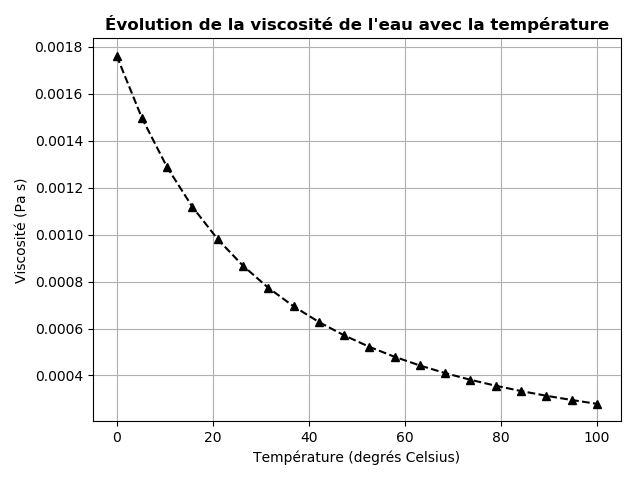
\includegraphics[width=0.7\linewidth]{figures/viscosity}
\end{itemize}
\end{bclogo}
\section*{Exercice 3 : Diffraction par ouverture rectangulaire}
Considérons un faisceau de lumière monochromatique de longueur d'onde $\lambda$ éclairant une ouverture rectangulaire située dans un plan $(xOy)$. La largeur de l'ouverture $b$ est dans la direction $x$ et sa hauteur $h$ est dans la direction $y$.

L'intensité normalisée de lumière en un point $M$ situé sur un écran ($E$) et à une distance $D$ de la fente peut s'écrire comme suit :
\begin{equation}
\dfrac{I(x_{M}, y_{M})}{I_{0}} = \text{sinc}^{2}\left (B \cdot x_{M} \right)\,\text{sinc}^{2}  \left ( H \cdot y_{M} \right )
\label{Eq_1_3}
\end{equation}
%
où $H = \frac{\pi h}{\lambda D}$, $B = \frac{\pi b}{\lambda D}$.

\begin{itemize}
\item La largeur de la tache centrale dans la direction $x$ est inversement proportionnelle à la largeur de l'ouverture: $\Delta x = \frac{2 \lambda D}{b}$;
\item La largeur de la tache centrale dans la direction $y$ est inversement proportionnelle à la hauteur de l'ouverture : $\Delta y = \frac{2 \lambda D}{h}$.
\end{itemize}

Écrire la fonction Python \verb|DiffRect(lamda, b, h, D)| qui calcul $\Delta x$ et $\Delta y$ et affiche la figure de diffraction :
\begin{pyshell}
>>> DiffRect(lamda= 630*1.E-9, b= 2*1.E-5, h= 4*1.E-5, D= 2)
La largeur de la tache centrale dans la direction x :  12.6
La largeur de la tache centrale dans la direction y :  6.3
\end{pyshell}
\begin{figure*}[th!]
\centering
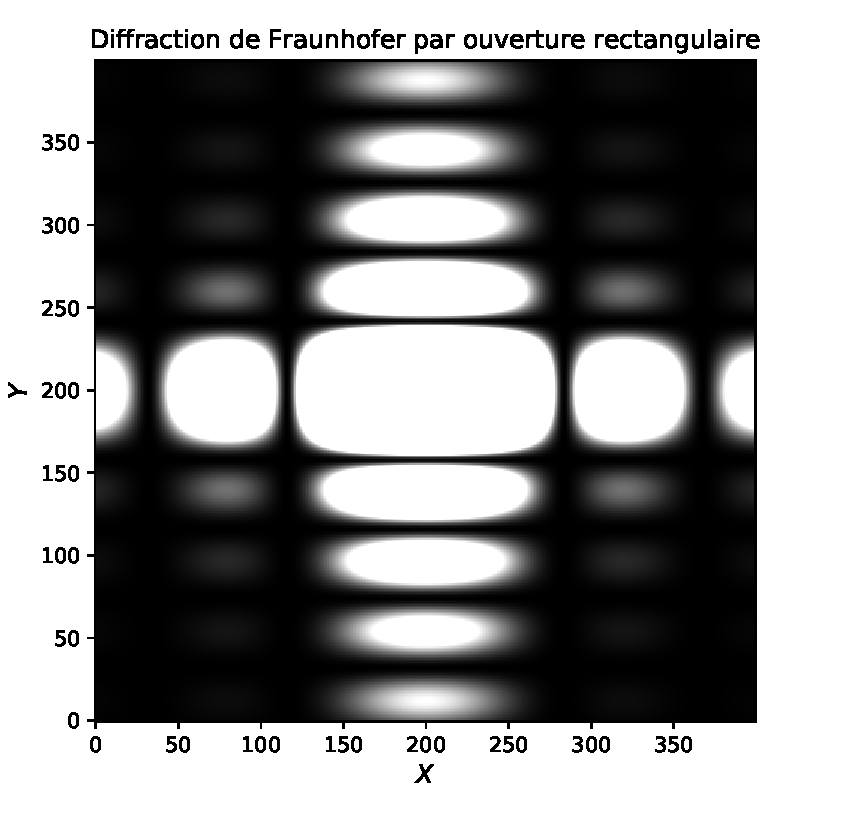
\includegraphics[width=0.55\linewidth]{figures/figureDiff}
\end{figure*}
\begin{bclogo}[logo=\bclampe, couleurBarre=green, noborder=true, couleur=yellow!10]{Indications.}
\begin{itemize}
\item[$\bullet$] `X,Y = np.meshgrid(x,y)`, avec \verb|x| et \verb|y| sont deux tableaux \verb|numpy|, est très utile pour évaluer des fonctions sur une grille.
\item[$\bullet$] \verb|plt.imshow(X)| afficher une image, à savoir des données sur une trame régulière 2D.
\end{itemize}
\end{bclogo}
\end{document}
